\documentclass[conference]{IEEEtran}
% \usepackage{../FinalYearProjectReport}

% packages for apendicies
\usepackage{color}
\usepackage{listings}
\definecolor{gray}{rgb}{0.4,0.4,0.4}
\definecolor{darkblue}{rgb}{0.0,0.0,0.6}
\definecolor{cyan}{rgb}{0.0,0.6,0.6}

\lstset{
  basicstyle=\ttfamily,
  numbers=left,
  columns=fullflexible,
  showstringspaces=false,
  commentstyle=\color{gray}\upshape
}

\lstdefinelanguage{JavaScript}{
  keywords={typeof, new, true, false, catch, function, return, null, catch, switch, var, if, in, while, do, else, case, break},
  keywordstyle=\color{blue}\bfseries,
  ndkeywords={class, export, boolean, throw, implements, import, this},
  ndkeywordstyle=\color{darkgray}\bfseries,
  identifierstyle=\color{black},
  sensitive=false,
  comment=[l]{//},
  morecomment=[s]{/*}{*/},
  commentstyle=\color{purple}\ttfamily,
  stringstyle=\color{darkblue}\ttfamily,
  morestring=[b]',
  morestring=[b]"
}

% packages for references
\usepackage{cite}
\usepackage{url}


% uncomment this line to double line spacing for proof reading
% \linespread{2}

% packages and settings for graphics
\usepackage{float}
\usepackage[pdftex]{graphicx}
\graphicspath{{./images}}
\DeclareGraphicsExtensions{.png}
\usepackage[final]{pdfpages}

\usepackage{relsize}
\relscale{1.1}


\title{Event Syndication and Dissemination}
\author{
  \IEEEauthorblockN{Christopher Morgan}
  \IEEEauthorblockA {
    Department of Electrical and Computer Engineering \\
    University of Auckland, Auckland, New Zealand
    }
}

\hyphenation{and-roid}


\begin{document}

\begin{titlepage}


\vspace*{20em}
\centering

{
	\large
	Department of Electrical and Computer Engineering\\
	Part IV Research Project Report\\
	2015

	\vspace{3em}

	\LARGE
	Event Syndication and Dissemination\\
}

\vspace*{4em}

Christopher Morgan, Matthew Dyer \\
Sathiamoorthy Manoharan

\vspace*{\fill}


\pagebreak
\vspace*{\fill}

{
	\Large 
	Declaration of Originality
}

\hspace{5em}

This report is my own unaided work and was not copied from nor written in collaboration with any other person.

Name: Christopher Morgan

\vspace*{\fill}
\end{titlepage}

\maketitle

\begin{abstract}
Currently, conference event information is stored and distributed in a non-standardised manner. This is either a pdf, mobile application or website, and a new instance of one needs to be created for each event. The event syndication and dissemination schema proposes a standardised way of storing this information. The schema maintains 100\% of schedule information from all conferences translated. A prototype web application has been made to realise the schema and evaluate it's effectiveness. Use of the prototype web application has proven that Open Conference Format performs better than traditional conference schedule viewers.
\end{abstract}


\section{Introduction}
The state of conference, convention and summit schedules are scattered. The format they come in is inconsistent, either a PDF, website or proprietary mobile application. These schedules are often poorly executed and leave a lot of room for improvement.

There are existing popular conference management systems such as OpenConf\cite{openconfWebsite}. These systems do a good job of the organisation and creating of conferences schedules, however their viewer applications leave much to be desired. What we're trying to do is create an open exchange format to separate the concerns of creating the conference schedule and viewing it. This separation splits the problem of managing conferences into three parts; creation, syndication and dissemination, and interaction. Our project focuses on the syndication and dissemination of these conference events, leaving their creation and interaction to other parties. However, in order to demonstrate the work we've done a reference prototype application was made.

In this report we will propose a standard schema for such events and discuss example applications that consumes event information compliant with the schema. Conference organisers will be able to use this schema to disseminate schedules that will then be viewed and interacted with on a diverse range of platforms.

\subsection{Conference schedules today}
Conference schedules come in a variety of formats; PDFs, mobile applications and websites. Professional conferences such as Google IO\cite{googleIO2015}, Embedded Linux Conference\cite{embeddedlinuxconference2015} and Apple WWDC\cite{appleWwdc2014} do it right. They provide an easy platform for attendees to find events, plan their schedules and receive updates. However, these are single use or proprietary systems behind a pay wall.

On the flip side, many academic conferences fail to provide schedules in easy to use formats. For example, IEEE conference schedules\cite{ieeePSC2015,ieeeICC2015,ieeeIMC2014} leave a lot to be desired. ICFICE 2015\cite{icfice2015} is a great example of how complicated these schedule views can be. The schedule largely consists of references to information located elsewhere in the document. Each seminar has a key that is references in the schedule grid. While looking up conferences based on their time is straightforward, looking up when and where a seminar from the key is time consuming and frustrating.

These PDF schedules have another major flaw, the lack of support for mobile devices. Viewing a PDF on a computer screen or printing it off is passable, but on a mobile phone the schedules are horrible. This issue has been a motivation throughout the entire project, from technology used when defining the format to how our reference application is architectured.

\subsection{Report structure}
To begin with, we'll cover the creation of Open Conference Format (OCF). This will include: the technologies used, motivations behind the choices made, where data was extracted from and how we determined it's validity. From there, we'll moved onto the reference viewer application. We'll discuss the technologies used, system architecture and problems faced. Then we'll discuss how we evaluated our work, what we plan to do in the future and finally, the conclusions drawn from this project.

\section{Creating a schema}

\subsection{XML vs. JSON}
Choosing a technology to represent the proposed schema required research into industry standards, trends in web technologies as well as standard library support in a multitude of languages. We looked into three candidates JSON (JavaScript Object Notation) and XML (eXtensible Markup Language).

\subsubsection{XML}
When we started this project, XML was the technology that our supervisor recommended we use. It's understandable that it should be the obvious choice, as it is the most widely used resource type in APIs\cite{maleshkova2010investigating}. XML is mature language, first released in 1996 and is used extensively by Microsoft and integrates well into .Net and Java applications.

XSD (XML Schema Definition) is the language used to describe XML schemas and is what would have been used if XML was chosen. The XSD, like most schema definition languages enables the creation of data types, inheritance and validation of data. One of the main inspirations of this project, RSS (Rich Site Summary or Really Simple Syndication) is defined using XSD along with many other XML based data transfer specifications.

\subsubsection{JSON}
Over the last few years, use of JSON in transferring over the internet and storing data as been increasing in popularity as seen in figure~\ref{fig:JSON_XML_all_time}. Not only this, but new services offering XML are decreasing as shown in figure~\ref{fig:JSON_XML_jan_2013}.

\begin{figure}[h]
	\centering
	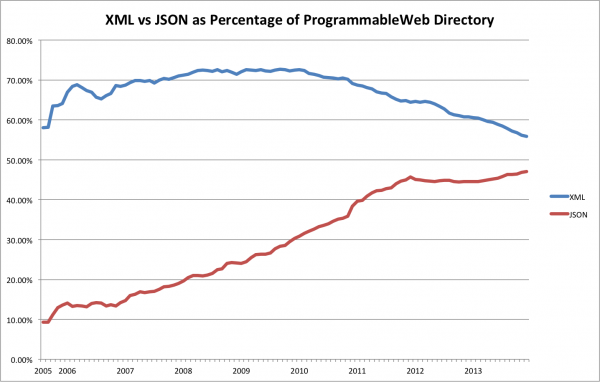
\includegraphics[scale=0.37]{images/xml_json_all_time.png}
	\caption{Overall XML vs. JSON Usage\protect\cite{duvander2013json}}
	\label{fig:JSON_XML_all_time}
\end{figure}

\begin{figure}[h]
  \centering
  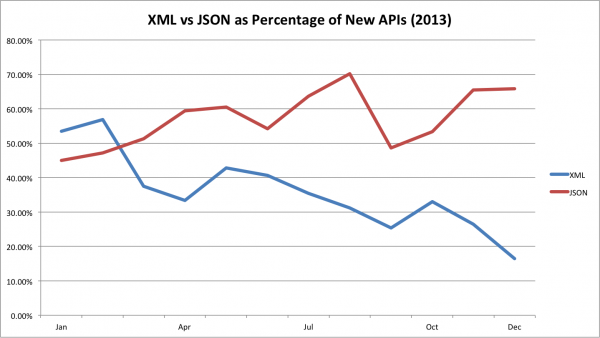
\includegraphics[scale=0.37]{images/xml_json_jan_2013.png}
  \caption{January 2013 New XML vs. JSON Usage\protect\cite{duvander2013json}}
  \label{fig:JSON_XML_jan_2013}
\end{figure}

This is in part due to the increase in the usage of front end web application frameworks such as React, AngularJS, Ember.js and Backbone.js. As such, this shift in usage is no surprise as JSON is easier, faster and cleaner \cite{hellstrom2012querying,lin2012comparison,nurseitov2009comparison} than XML when working with using it's namesake, JavaScript. As one of the primary outcomes of this project is to create an example web application, this ease of use plays heavily when choosing which technology to use.

JSON Schema \cite{galiegue2013json} is currently a work in progress specification. Draft 4 has been out for a few years and contains everything necessary to define a JSON schema that can describe conference events. Even though this it is still in draft, with third party library support in many languages \cite{galiegue2013inplementations} and having been unchanged in 2 years it is sufficiently mature to use in a university project.

\subsection{Prototyping the schema}
The first stage of the project was developing a schema to encapsulate conference information. To gather requirements for schema, a multitude of academic conference schedules were examined. This included, but was not limited to:
\begin{itemize}
\item International Conference on Future Information \& Communication Engineering 2014
\item Pacrim 2013
\item International Symposium on Information Theory and Its Applications
\item Department of Electrical and Computer Engineering, Part IV Project Seminar 2014
\end{itemize}

See listing~\ref{lst:jsonSchema} on page~\pageref{lst:jsonSchema} for the full proposed schema. The schema will evolve over time and can be versioned accordingly, allowing easier future development and the building of more advanced schedules.

\begin{figure}[h]
  \centering
  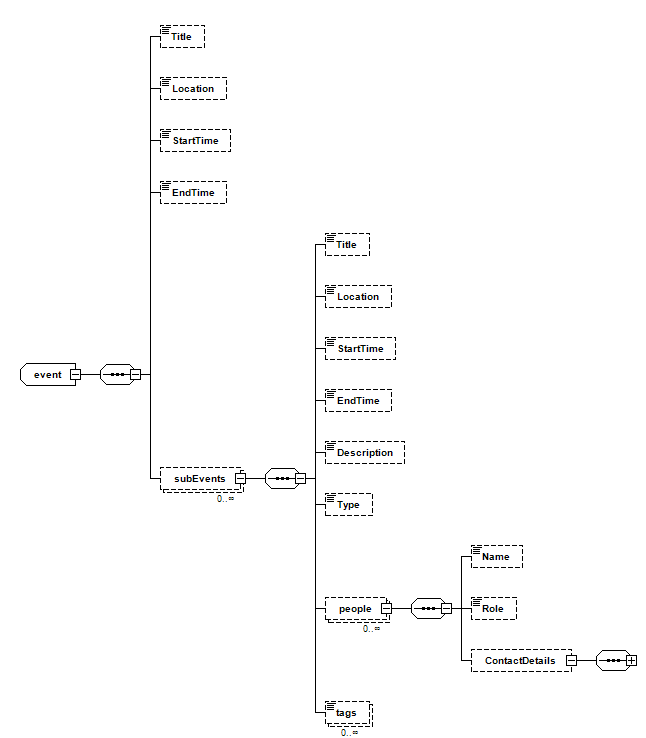
\includegraphics[scale=0.475]{images/schema_1.png}
  \caption{Open Conference Format}
  \label{fig:schema_1}
\end{figure}

\section{Building a reference application}

To fully realise Open Conference Format, a reference implementation of a viewer application was needed. Creating the unified standard is all well and good, but if we can't show an improvement over existing systems it would be difficult to gain momentum with conference organisers and application developers.

\subsection{Technology}
Starting from scratch and creating a compelling application with plain JavaScript, HTML and CSS is a tough task and not in scope for this project. Fortunately, there is a plethora of frameworks and tools that can be leveraged when creating modern web applications.

Keeping with the theme of using modern or emergent technology, we opted to create a single page web application for our prototype. This would allow us to target as many devices as possible, creating the application with both desktop and mobile viewing in mind.

\subsubsection{AngularJS}
Supporting all the functionality we desired and with a strong community behind it, AngularJS was the obvious choice when choosing a frontend framework. Before starting this project, I'd had a few months of experience with it and knew that it would be easy use.

\begin{figure}[h]
  \centering
  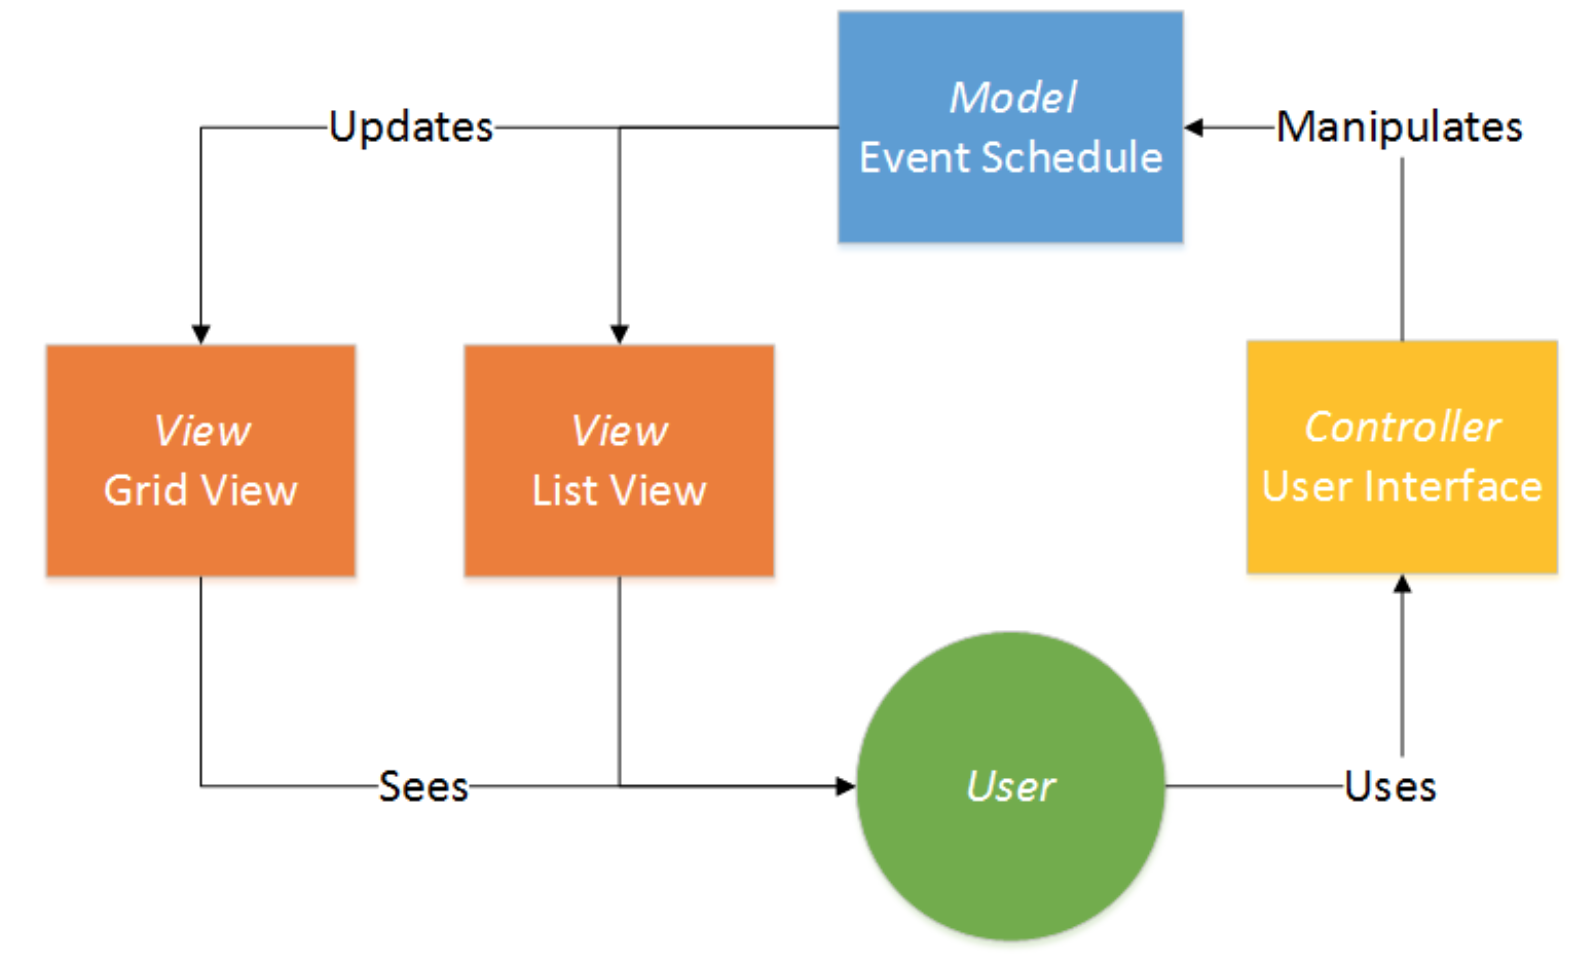
\includegraphics[scale=0.28]{images/arch_1.png}
  \caption{MVC architecture view}
  \label{fig:arch_1}
\end{figure}

Using the services architecture AngularJS, we were able to create parts of the system with a large amount of interoperability. Paired with a MVC (Model View Controller) architecture, it was easy to create multiple views for the same information, something that we ended up needing to do.

Dependency injection was utilised to add third-party libraries, including easy access to local browser storage. This storage was used to persist application state between user sessions.

To create a truly interactive web application, two-way data binding was used to adjust displayed data as the user interacted with it. This was used to implement the search functionality and custom schedule, as the user types in the search bar, the seminars filter simultaneously.

\subsubsection{Node.js}
Originally, there was no need for a webserver, only static assets were needed to use the application. However, when we implemented vCard contact saving and iCal calendar exporting, the need arose for us to serve dynamic files that a frontend application simply couldn't do.

Node.js is a simple serverside JavaScript engine. It allows us to program both the frontend and backend in the same language, reducing development friction. The web application framework, ExpressJS was used to handle HTTP requests and static file serving.

\subsection{Design}
We designed the application to be simple and straight forward, focusing more on functionality rather than form. That being said, the CSS framework Bootstrap was used to make simple styling easy and visual appealing. We were able to use a lot of the predefined classes when styling the interface, making the process much easier.

\subsubsection{Grid view}
Initially, we took design inspiration from existing conference schedules and laid everything out in a grid pattern. Seminars were sorted by time vertically and location horizontally, essentially forming streams of events. The view can be seen in figure~\ref{fig:grid_view} on page~\pageref{fig:grid_view}. This would provide familiarity for users of traditional schedules as well as form a base for how the user interacted with the information.

We found that displaying all the schedule information in the grid view was cluttered and decided to hide most of the detail until it was relevant to the user, much like how complicated conference schedules had key lookup tables. When event titles are clicked, a detail modal pops up. In this modal, the user can save the seminar to their personal schedule, save speakers contact details and open speaker details with contextual links. For example, if one of the contact details is their email address, clicking on said address would launch an email client and start a draft email to their address.

To easily find seminars, search functionality is included in the app. The search looks all the schedule information, allowing the user to find seminars based on title, speakers, theme and time.

\subsubsection{List view}
While the grid view works well on desktop computers, the layout does not work well on mobile devices. It made sense to have a separate, more mobile optimised view as well. Mobile phones have a more vertical orientated interface meaning that schedule would need to conform to that kind of layout. The list view can be seen in figure~\ref{fig:list_view} on page~\pageref{fig:list_view}.

The list view contains all the functionality of the grid view and was very easy to adapt due to the architectural choices we made early in the project. It utilises responsive CSS, allowing it to scale to any display size smoothly.

\section{Evaluation}

Drafting an event syndication schema and implementing consuming applications is all well and good, however validating the quality, usability and completeness of what was done requires objective evaluation. Conference schedules already exist, this project isn't trying to change how they are structured or determined but rather provide a compliant data format for organisers to utilise in order to distribute schedule information.

\subsection{Format interchange}
To evaluate the outcome of this project, conferences from in a variety of formats and structures were translated into Open Conference Format. If conference information is unable to be translated to fit the schema, that would weigh negatively. Not many conference systems have exportable data, however OpenConf does. We wrote a service in the web application that can convert OpenConf data to OCF with 100\% data retention. Schedule data was also imported from academic and professional conferences, again with 100\% data retention.

\subsection{Case study}
To evaluate how well Open Conference Format and the reference web application performs, a case study was carried out with the ECE Part IV Project Seminar Schedule from 2014. The schedule information was translated from the original PDF form into OCF. Industry professionals were asked to evaluate the usability and performance of the reference application in comparison with the PDF version.

\subsubsection{Professional evaluation}
Professionals were asked to find events with differing views of the schedule. Primarily, the viewer application's list and grid views were compared to a digital copy of the PDF. The expected results were that the PDF would perform poorly and the list and grid view would perform about the same. However, the results shown in figure~\ref{fig:eval_results} show that list view performed just as poorly as the PDF wile the grid view performed roughly twice as well.

\begin{figure}[h]
  \centering
  \begin{tabular}{ l r }
    \hline
    Schedule Type & Mean Time (seconds) \\
    \hline
    PDF           & 21.0                \\
    Grid View     & 11.3                \\
    List View     & 22.4                \\
  \end{tabular}
  \caption{Professional Evaluation Results}
  \label{fig:eval_results}
\end{figure}

The professionals we also asked to complete a survey, detailing their experience with the various schedule views. The feedback showed that users preferred the aesthetics of the list view compared to the grid view. A few of the participants detailed that they couldn't initially find the search bar, this lined up with significantly longer task times. In response to this, the search bar was moved to the traditional position of the top right corner. They also remarked how they much preferred the interactive web viewer compared to the PDF, saying that the adaptive content helped them identify the information they were seeking.

\section{Future work}

\subsection{Evolving schema}
How conferences are organised and their format will change over time. In order for Open Conference Format to survive it must evolve as well. The versioning system built into OCF can be used to easily tweak the schema and adjust viewer applications while keeping backwards compatibility.

\subsection{Translation from additional formats}
Currently, we're only able to convert from OpenConf to OCF. This is hardly due to the closed source nature of the majority of conference schedule creation systems. Expanding this functionality by being able to import schedules from an increased amount of formats would reduce the friction of conferences moving to use our format.

\subsection{Open source project contribution}
There are a number of open source conference management systems. Most notably Open Conference Systems\cite{ocsWebsite}. Having open source solutions use our schema would greatly increase the chances of large academic conferences using our format as well. Due to the open source nature of the products, submitting pull requests would be trivial.

\subsection{Native mobile applications}
We were originally wanting to develop native applications for both Android and iOS, however due to time constrains we were unable to. These applications could fully utilise the power of smart phones, integrating with the contacts manager, calendar and maps. These mobile applications would be more tailored to each platform and be more battery efficient.

Integration isn't limited to just first-party applications either. A native implementation could use services such as Uber and AirBnb to assist conference goers with transport and accommodation.

\section{Conclusion}
Current formats of conference schedule information is fractured, there is a need for a unifying format. We propose Open Conference Format as a solution, standard to be used in the syndication and dissemination of conference schedules. There are only advantages to translating schedules to OCF, with 100\% data retention and a significant increase in viewer application performance.

\section{Acknowledgments}
Dr. Sathiamoorthy Manoharan

Dr. Gerald Weber

Dr. Jing Sun

\bibliographystyle{IEEEtran}
\bibliography{interim_report}

\onecolumn
\appendix
\section{Schema}
\lstinputlisting[caption=JSON Schema Description, language=JavaScript, label={lst:jsonSchema}]{../../schema/esad.schema.json}

\section{Interface}
\begin{figure}[h]
  \centering
  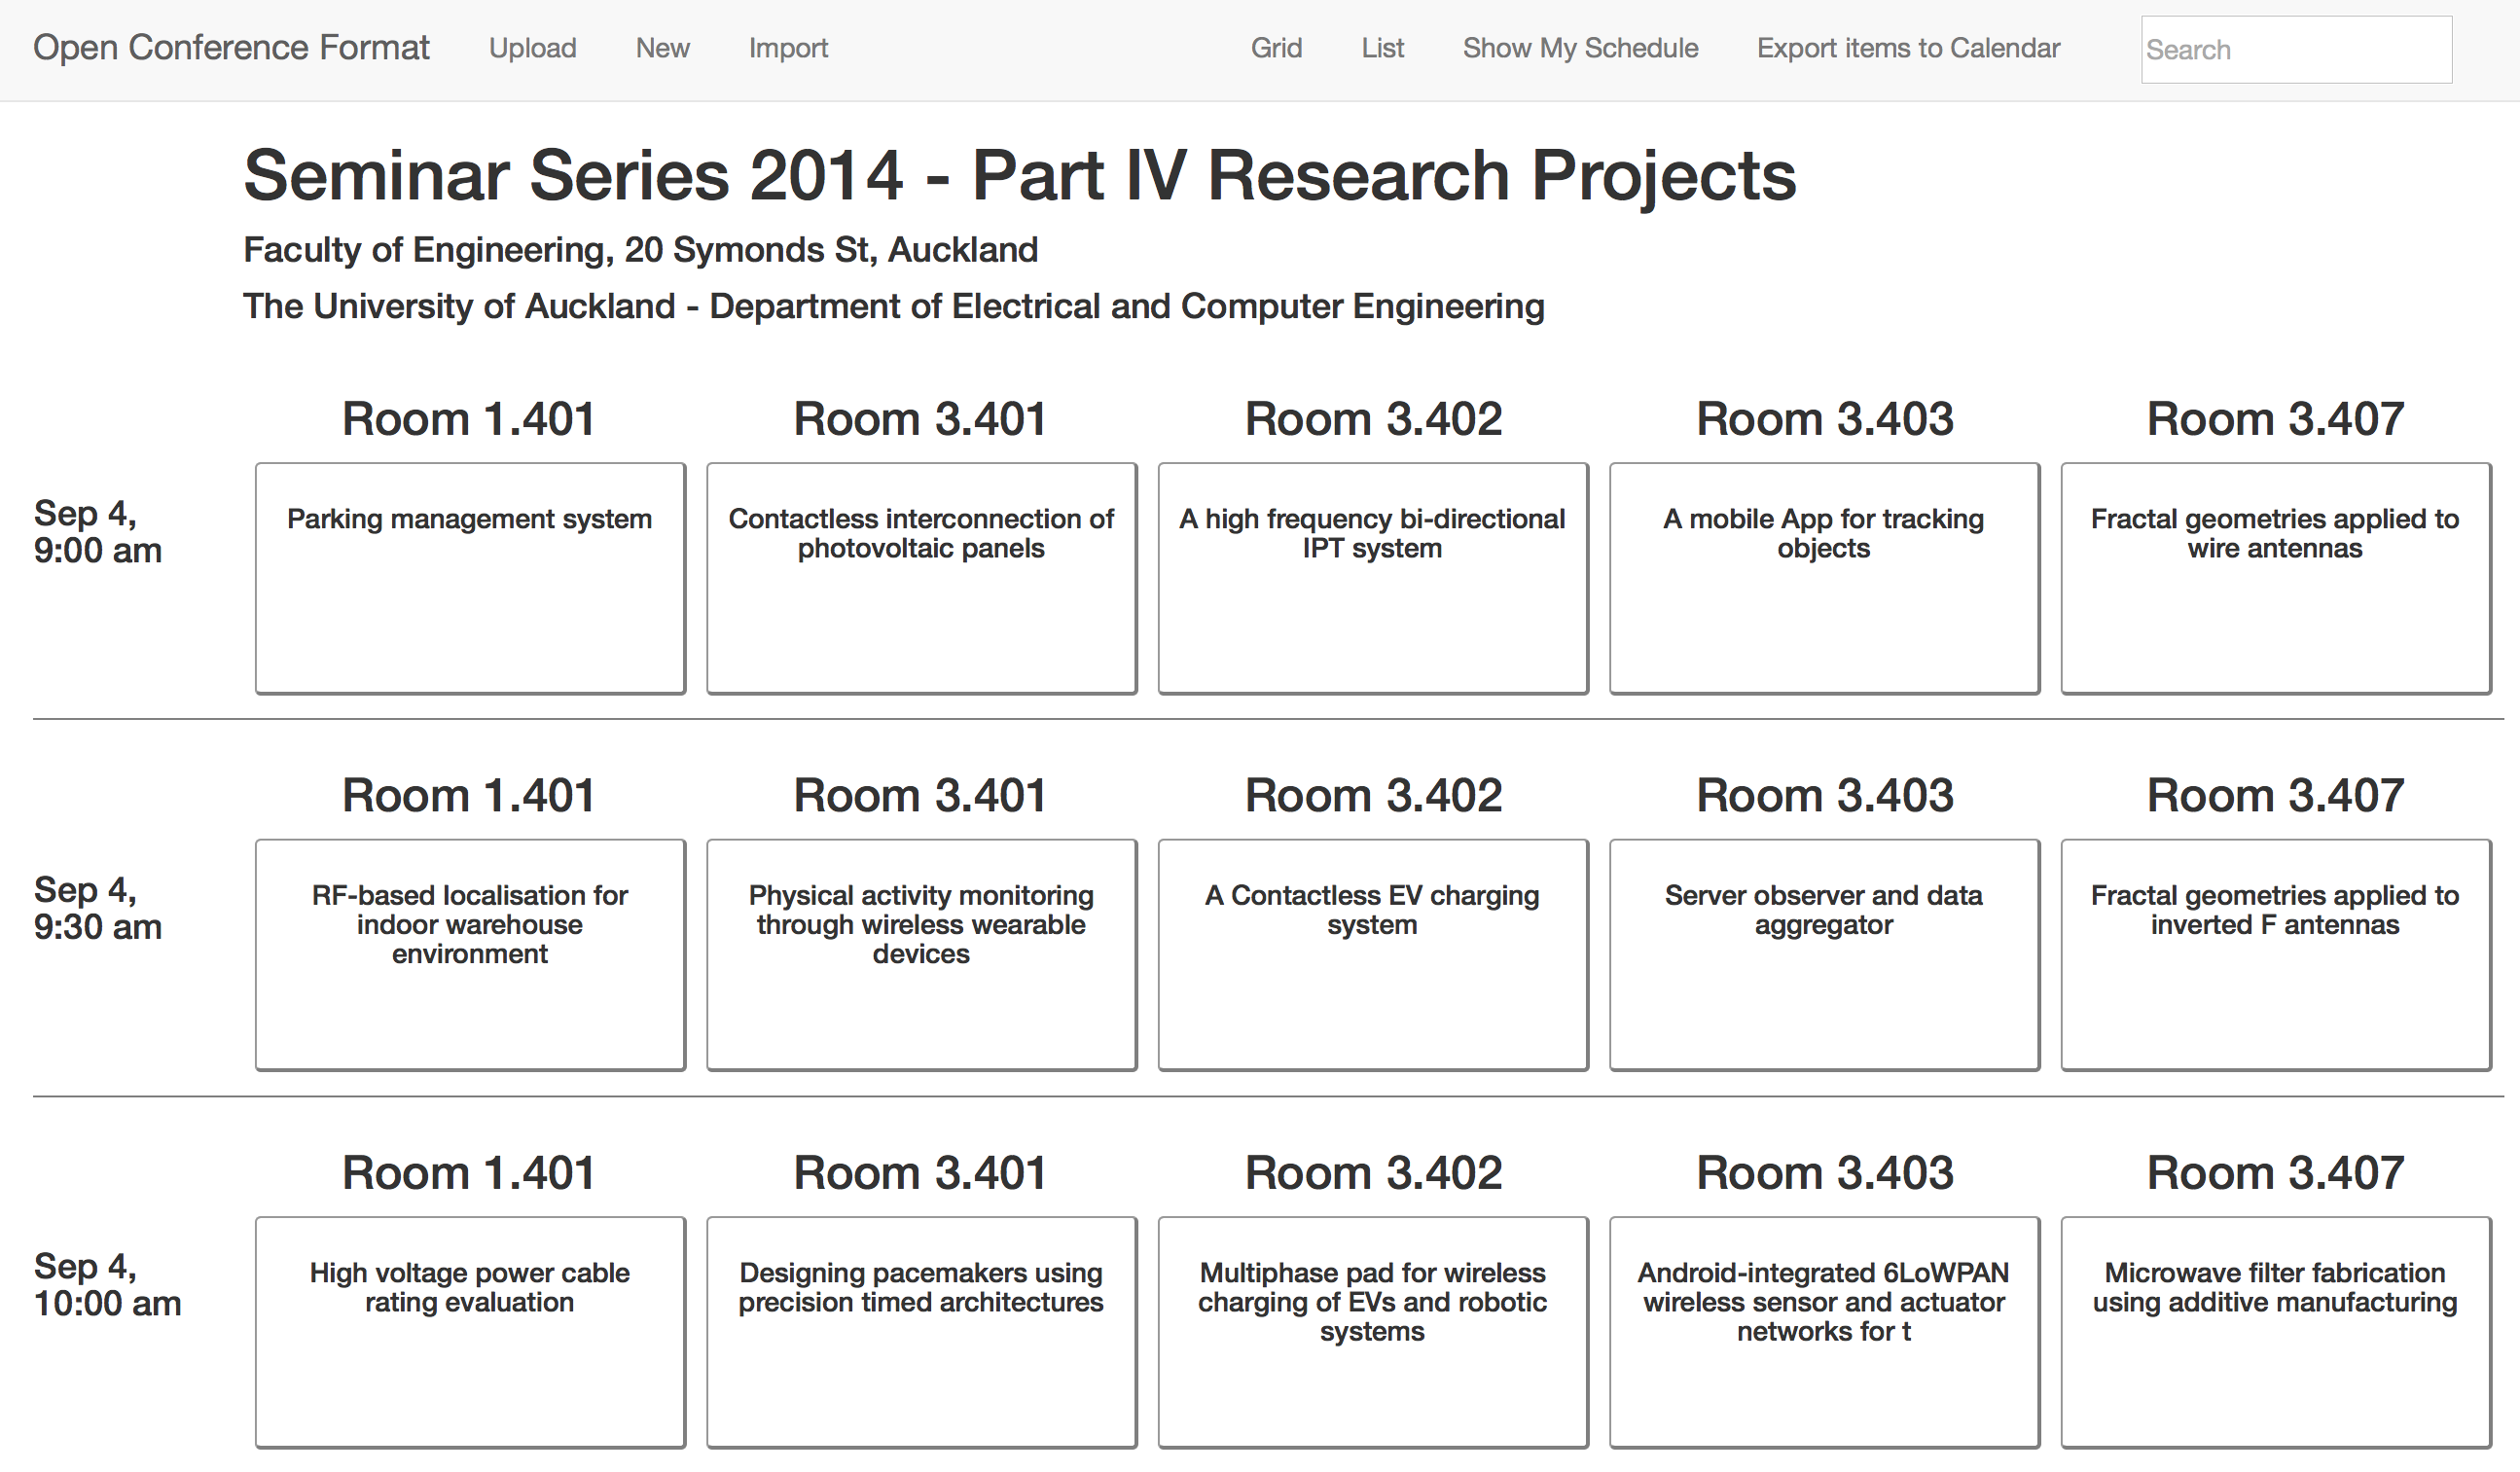
\includegraphics[scale=0.4]{images/grid_view.png}
  \caption{Grid view}
  \label{fig:grid_view}
\end{figure}

\begin{figure}[h]
  \centering
  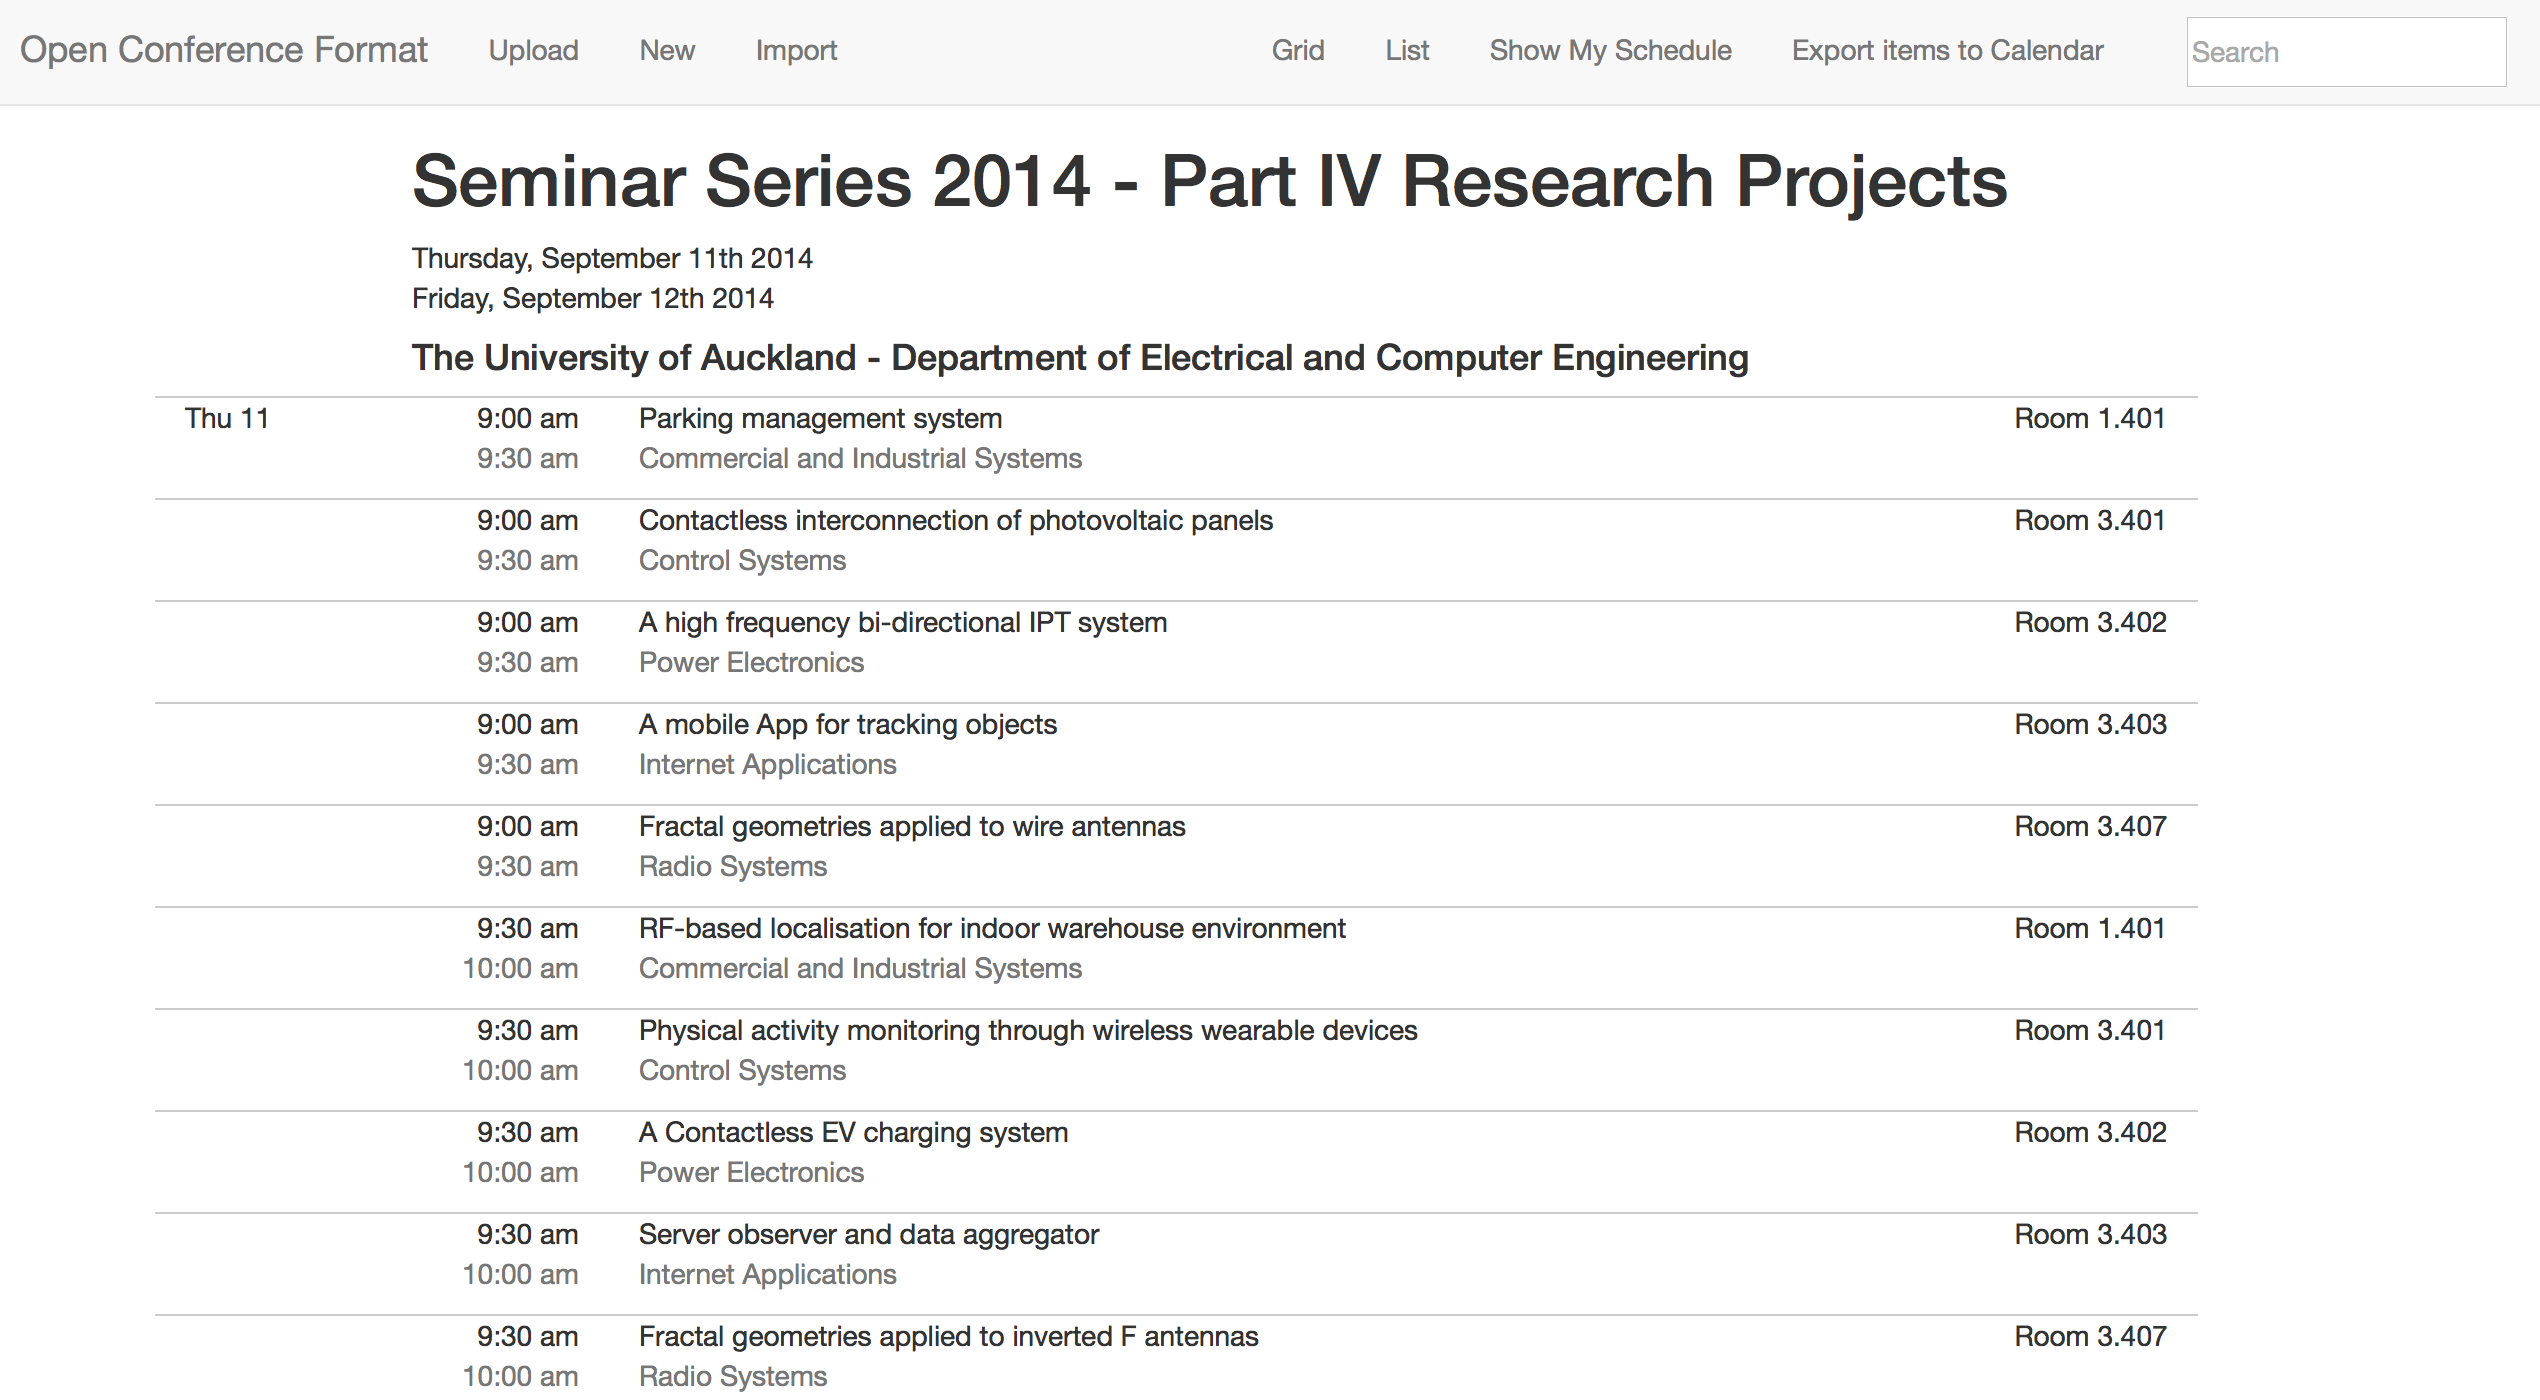
\includegraphics[scale=0.4]{images/list_view.png}
  \caption{List view}
  \label{fig:list_view}
\end{figure}

\end{document}